\documentclass{article}

\usepackage[margin=1in]{geometry}
\usepackage{amsmath,amsthm,amssymb}
\usepackage{bbm,enumerate,mathtools}
\usepackage[hidelinks]{hyperref}
\usepackage{tikz}
\usetikzlibrary{matrix, arrows}

\newenvironment{problem}[2][Problem]{\begin{trivlist}
\item[\hskip \labelsep {\bfseries #1}\hskip \labelsep {\bfseries #2.}]}{\end{trivlist}}
\newenvironment{note}[1][Note.]{\begin{trivlist}
\item[\hskip \labelsep {\bfseries #1}]}{\end{trivlist}}
\newenvironment{problempart}[1]{\begin{trivlist}\item[\textbf{Part #1.}]}{\end{trivlist}}


\begin{document}

\title{Differential Geometry: Homework 5}
\author{Peter Kagey}

\maketitle

% -----------------------------------------------------
% First problem
% -----------------------------------------------------
\begin{problem}{1}
  Let $M = f^{-1}(y)$ be the primage of a regular value
  $y \in \mathbb{R}^{N - m}$ of a (smooth) submersion
  $f\colon \mathbb{R}^N \rightarrow \mathbb{R}^{N-m}$.
  \begin{enumerate}[(a)]
    \item Let $
      \widetilde{TM} =
      \{(x, v) \in \mathbb{R}^N \times \mathbb{R}^N : x \in M, v \in \ker df_x\}
    $. Show that as defined $\widetilde{TM}$ is a smooth submanifold of
    $\mathbb{R}^N \times \mathbb{R}^N$ of dimension $2m$.
    \item Prove that there is a diffeomorphism between $\widetilde{TM}$ and the
      \textit{tangent bundle of $M$}  as defined in class: \[
        \widetilde{TM} \cong TM
      \] in a manner compatible with projection to $M$.
  \end{enumerate}
\end{problem}

\begin{proof} \text{} \\
  \begin{enumerate}[(a)]
    \item
      Because $M$ is the preimage of a smooth submersion, by the implicit
      function theorem, $M$ is an $m$-dimensional manifold, with maximal atlas $
        \mathcal{A}_M = \{\,
          (U^M_i, \phi^M_i\colon U^M_i \rightarrow \mathbb{R}^m)
        \,\}_{i \in I}
      $.\\~\\
      % For an arbitrary open subset $U \subset \mathbb{R}^n \times \mathbb{R}^n$,
      Let $\pi$ be the projection onto the first $N$ coordinates, then \[
        \phi_i \circ \pi\colon \underbrace{\pi^{-1}(U_i)}_{\subset \mathbb{R}^{2m}} \rightarrow \mathbb{R}^m
      \] is the composition of smooth maps, so is smooth.

      Similarly, because $f$ is a submersion,
      $df_x\colon \mathbb{R}^N \rightarrow \mathbb{R}^{N - m}$
      (which is a linear map) is a surjection, and so is of full rank. Therefore
      $\ker df_x \cong \mathbb{R}^m$ via some isomorphism $\psi_x$.
      Thus we can construct an atlas for $\widetilde{TM}$ where each chart
      consists of the set $\widetilde{U}_i = U_i \times \mathbb{R}^m$ together
      with the function \[
        \widetilde{\phi}_i\colon \widetilde{U}_i \rightarrow \mathbb{R}^{2m}
        \text{ which sends }
        \underbrace{(x, v)}_{\in U_i \times \mathbb{R}^m} \mapsto \underbrace{(\phi(x), \psi_x(v))}_{\in \mathbb{R}^{2m}}
      \] and so $\widetilde{TM}$ is a submanifold of dimension $2m$.
    \item
      (I'm not sure I understand this problem.)
      \\
      As defined in class, \[
        TM = \bigsqcup_{p \in M} T_pM = \{\, (p, \vec{v}) : \vec{v} \in T_pM \,\}.
      \]
      By using the second extrinsic defintion of a tangent space
      (given in lecture), $T_pM = \ker df_p$, so the identity map is a perfectly
      good diffeomorphism from $\widetilde{TM}$ to $TM$. (In order to use a
      different definition, one must only construct a diffeomorphism between the
      desired definition and the second extrinsic definition.)
  \end{enumerate}
\end{proof}

% -----------------------------------------------------
% Second problem
% -----------------------------------------------------
\pagebreak

\begin{problem}{2}
  Let $M^m$ be a manifold of dimension $m$ and $p \in M$ a point. Recall that
  $\mathcal{F}_p \subset C^\infty(p)$ is the ideal of germs of functions on $M$
  which vanish at $p \in M$. Let $\mathcal{F}_p^k$ be the ideal of $C^\infty(p)$
  generated by $f_1 \hdots f_k$, where $f_i \in \mathcal{F}_p$.
  \begin{enumerate}[(a)]
    \item
      Prove that, in every set of local coordinates $(x_1, \hdots , x_k)$
      around the point $p$, an element $f \in \mathcal{F}^k_p$ has a Taylor
      expansion which vanishes to order $k$. You may assume a version of
      Taylor’s approximation theorem stated in class.
    \item Compute the dimension of $\mathcal{F}_p^k/\mathcal{F}_p^{k+1}$.
    \item Construct a smooth manifold along with a map to $M$,
    $E \xrightarrow{\pi} M$ whose ``fiber'' $E_p = \pi^{-1}(p)$ at the point
    $p \in M$ is $\mathcal{F}_p^1/\mathcal{F}_p^3$.
  \end{enumerate}
\end{problem}

\begin{proof} $ $
  \begin{enumerate}[(a)]
    \item
      Because each germ $f_\ell \in \mathcal{F}_p$ consists of representatives that
      agree on a small neighborhood around $p$, all representatives have
      identical Taylor expansions \[
        f_\ell(x) = \underbrace{f_\ell(p)}_0 + \sum_i a_{\ell,i} x_i
          + \sum_{i,j} g_{\ell,ij}(x) x_i x_j
      \] where
      $a^\ell_i, a^\ell_{ij} \in \mathbb{R}$, $g^\ell_{ij} \in C^\infty(p)$, and
      $f_\ell(p) = 0$ by defintion of $\mathcal{F}_p$.
      Then an element of $\mathcal{F}_p^k$ is generated by \[
        f_1 f_2 \cdots f_k =
          \left(\sum_i a_{1,i} x_i + \sum_{i,j} g_{1,ij}(x) x_i x_j\right) \cdots
          \left(\sum_i a_{k,i} x_i + \sum_{i,j} g_{k,ij}(x) x_i x_j\right)
      \] and therefore each term of each element in the generating set vanishes
      to order $k$, so the Taylor expansion of any element in $\mathcal{F}_p^k$
      vanishes to order $k$.
    \item Each equivalence class of germs in
      $\mathcal{F}_p^k/\mathcal{F}_p^{k+1}$ consists of functions whose Taylor
      expansions vanish to order $k$, and that are equivalent if their order $k$
      terms are identical.
      Thus the dimension of $\mathcal{F}_p^k/\mathcal{F}_p^{k+1}$ is $m^k$,
      because there are $m^k$ ways of choosing $k$ elements from
      $\{ x_1, \hdots, x_m \}$ with replacement, and so there are $m^k$ possible
      coefficients $a_{i_1 \hdots i_k}$ for the order $k$ term.
    \item
      Let \[
        E = \bigsqcup_{p \in M} E_p
          = \{\, (p, \mathcal{F}_p/\mathcal{F}_p^3) : p \in M \,\}.
      \] and let $\pi: E \rightarrow M$ map $E_p \mapsto p$.
      \\
      Denote the atlas of $M$ by $\mathcal{A}_M = \{ (U_i, \phi_i) \}_{i \in I}$,
      and let $\widetilde{U}_i = \pi^{-1}(U_i)$ (that is, the germs of all
      functions that vanish at a point in $U_i$ modulo terms of order 3 and
      greater), and let
      $\widetilde{\phi}_p: \widetilde{U}_p \rightarrow \mathbb{R}^{2m + m^2}$ map
      (the germ of) a function to the point that it vanishes ($p$) at and the
      coefficients (of order 1 and 2) in its Taylor expansion centered at $p$
      (in local coordinates with respect to $\phi$):
      \[
        [f] = \left[
          \sum_{i=1}^m a_i x_i + \sum_{i=1}^m\sum_{j=1}^m a_{ij} x_i x_j
        \right] \mapsto
        (\underbrace{p_1, \hdots, p_m}_{\in \mathbb{R}^m}, \underbrace{
        a_1, \hdots, a_m, a_{11}, a_{12}, \hdots a_{1m}, a_{21}, \hdots a_{mm}
        }_{\in \mathbb{R}^{m + m^2}}).
      \]
  \end{enumerate}
\end{proof}

% -----------------------------------------------------
% Third problem
% -----------------------------------------------------
\pagebreak

\begin{problem}{3}
  Let $f\colon M \rightarrow N$ be a smooth map between manifolds. Prove that
  the following diagram commutes:

  \centering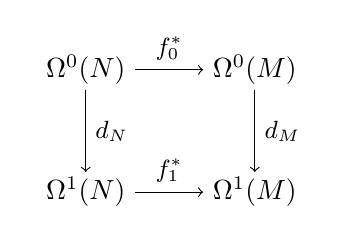
\begin{tikzpicture}[description/.style={fill=white,inner sep=2pt}]
    \matrix (m) [matrix of math nodes, row sep=3em,
    column sep=2.5em, text height=1.5ex, text depth=0.25ex] {
      \Omega^0(N) & \Omega^0(M) \\
      \Omega^1(N) & \Omega^1(M) \\
    };
    \path[-,font=\small]
      (m-1-1) edge[->] node[auto] {$f^*_0$} (m-1-2)
      (m-1-1) edge[->] node[auto] {$d_N$} (m-2-1)
      (m-2-1) edge[->] node[auto] {$f^*_1$} (m-2-2)
      (m-1-2) edge[->] node[auto] {$d_M$} (m-2-2);
  \end{tikzpicture}


\end{problem}

\begin{proof} \text{} \\
  It is sufficient to show that $d_M(f^*_0(g)) = f^*_1(d_N(g))$ for all
  functions $g \in \Omega^0(N) = C^\infty(N)$.\\~\\
  Thus taking an arbitrary function $g \in C^\infty(N)$ and arbitrary point
  $p \in M$, the ``upper right'' path of the diagram yields a contangent vector
  in $T^*M$:
  \begin{align*}
    d_M(f^*_0(g))(p)
    &= d_M(g \circ f)(p) \\
    &= (p, d(g \circ f)_p) \\
    &= (p, [g \circ f - g \circ f(p)]) \in T^*M.
  \end{align*}
  Similarly, evaluating the ``lower right'' path of the diagram with the same
  function and point yields the same cotangent vector: \begin{align*}
    f^*_1(d_N(g))(p)
      &= (p, f^*(d_N(g)_{f(p)})) \\
      &= (p, f^*[g - g(f(p))]) \\
      &= (p, [g \circ f - g \circ f(p)]) \in T^*M.
  \end{align*}.

  Therefore $d_M(f^*_0(g)) = f^*_1(d_N(g))$, and the diagram commutes.
\end{proof}

% -----------------------------------------------------
% Fourth problem
% -----------------------------------------------------
\pagebreak

\begin{problem}{4}
  Give a detailed proof that the cotangent bundle $T^*M$ is a smooth manifold
  and that the projection map $\pi\colon T^*M \rightarrow M$ is a smooth map.
\end{problem}

\begin{proof} \text{}\\
  Use the defintion of $T^*M$ from class: \[
    T^*M
      = \bigsqcup_{p \in M} T_p^*M
      = \{\, (p, v^*)\ |\ p \in M, v^* \in T_p^*M\,\}
  \] with a topology given by \[
    \mathcal{T}_{T^*M} = \{\, W \subset T^*M\ |\ \widetilde{\phi}_i(W \cap \widetilde{U}_i) \text{ is open in } \mathbb{R}^{2n} \text{ for all } i \in I \,\}
  \] where \begin{enumerate}[(a)]
    \item $\displaystyle \mathcal{A}_M = \{(U_i, \phi_i)\}_{i \in I}$ is $M$'s
      maximal atlas.
    \item $\displaystyle \pi\colon T^*M \rightarrow M$ is a map that sends
      $(p, \vec{v}) \mapsto p$.
    \item $\widetilde{U}_i = \pi^{-1}(U_i) \subset T^*M$
    \item $\widetilde{\phi}_i\colon \widetilde{U}_i \rightarrow \phi_i(U_i) \times \mathbb{R}^{m}$
      is a map that sends
      $(p, \vec{v}) \mapsto (\phi_i(p), d(\phi_i)_p(\vec{v}))$.
  \end{enumerate}
  Then the atlas on $T^*M$ is given by \[
    \mathcal{A}_{T^*M} = \{(\widetilde{U}_i, \widetilde{\phi}_i)\}_{i \in I}.
  \] \\~\\
  %
  It is sufficient to show that
  % (i) $\mathcal{T}_{T^*M}$ is actually a topology,
  (i) $\{\widetilde{U}_i\}_{i \in I}$ is an open cover of $T^*M$,
  (ii) $\mathcal{A}_{T^*M}$ has smooth transition maps, and
  (iii) $\pi\colon T^*M \rightarrow M$ is a $C^\infty$ map.

  \begin{enumerate}[(i)]
    % \mathcal{T}_{T^*M} = \{\, W \subset T^*M\ |\ \widetilde{\phi}_i(W \cap \widetilde{U}_i) \text{ is open in } \mathbb{R}^{2n} \text{ for all } i \in I \,\}
    % \item (?)\\
    %   \textbf{The empty set and the entire set are the in the topology.}
    %   \[\widetilde{\phi}_i(\emptyset \cap \widetilde{U}_i) = \widetilde{\phi}_i(\emptyset) = \emptyset \in \mathcal{T}_{\mathbb{R}^{2m}}\]
    %   \[
    %     \widetilde{\phi}_i(T^*M \cap \widetilde{U}_i)
    %     = \widetilde{\phi}_i(\widetilde{U}_i)
    %     = \phi_i(U_i) \times \mathbb{R}^m
    %     \in \mathcal{T}_{\mathbb{R}^{2m}}
    %   \]
    %   \textbf{The topology is closed under arbitrary union.}\\
    %   Suppose that $W_j \in \mathcal{T}_{T^*M}$, for $j$ in some index set $J$,
    %   that is $\widetilde{\phi}_i(W_j \cap \widetilde{U}_i)$ is open for all
    %   $i \in I$ and $j \in J$.
    %   \\
    %   \textbf{The topology is closed under finite intersection.}\\
    %   Suppose that $W, V \in \mathcal{T}_{T^*M}$, that is
    %   $\widetilde{\phi}_i(W \cap \widetilde{U}_i)$ and
    %   $\widetilde{\phi}_i(V \cap \widetilde{U}_i)$ are open in $\mathbb{R}^{2n}$
    %   for any arbitrary $i \in I$.
    %   Thus $\widetilde{\phi}_i(V \cap W \cap \widetilde{U}_i)$ is open, so
    %   $V \cap W \in \mathcal{T}_{T^*M}$.
    \item
      Let $(p, v*) \in T^*_pM$. Then there exists some $U_i$ such that
      $p \in U_i$ because the atlas $\mathcal{A}_M$ covers $M$. Take this $U_i$,
      and $\widetilde(U)_i = \pi^{-1}(U_i)$ is an open set which contains
      $(p, v*)$. Thus every point is in an open set, and
      $\{\widetilde{U}\}_{i \in I}$ is an open cover of $T^*M$.
    \item
      Suppose that $(\widetilde{U}, \widetilde{\phi})$ and
      $(\widetilde{V}, \widetilde{\psi})$ are charts from open subsets
      of $T^*M$ to $\mathbb{R}^{2n}$ with nonempty intersection.
      Then $\widetilde{\phi} \circ \widetilde{\psi}^{-1}\colon \mathbb{R}^{2n} \rightarrow \mathbb{R}^{2n}$
      maps \[
        (x, y) \xmapsto{\widetilde{\psi}^{-1}} (\psi^{-1}(x), d\psi^{-1}_x(y))
        \xmapsto{\widetilde{\phi}} (\phi \circ \psi^{-1}(x), d\phi_{\psi^{-1}(x)}(d\psi^{-1}_x(y))).
      \]
      $\phi \circ \psi^{-1}$ is a $C^\infty$ map because this is inherited
      from the $C^\infty$ transition maps on $M$, and $
      d\phi_{\psi^{-1}(x)}(d\psi^{-1}_x(y))$ is smooth because it is the
      derivative of the $C^\infty$ map
      \[d\phi_{\psi^{-1}(x)}(d\psi^{-1}_x(y)) = d(\phi \circ \psi^{-1})_x(y)\]
    \item
      By definition, $\pi$ is a $C^\infty$ map if for each point
      $(p, v*) \in T^*M$, there exists a chart $(U_i, \phi_i)$ around $p$ such
      that $
        \phi_i \circ \pi \circ \widetilde{\phi}_i^{-1}\colon
        \mathbb{R}^{2m} \rightarrow \mathbb{R}^m
      $ is smooth.
      However, $\phi_i \circ \pi \circ \widetilde{\phi}_i^{-1}\colon$ is simply
      the projection \[
        (x, y)
        \xmapsto{\widetilde{\phi}^{-1}_i} (\phi^{-1}_i(x), d(\phi^{-1}_i)_x(y))
        \xmapsto{\pi} \phi^{-1}_i(x)
        \xmapsto{\phi_i} x,
      \] and projections are smooth.
  \end{enumerate}
\end{proof}

% -----------------------------------------------------
% Fifth
% -----------------------------------------------------
\pagebreak

\begin{problem}{5}
  Let $f, g\colon M \rightarrow \mathbb{R}$ be smooth real-valued functions on a
  manifold $M$. Prove that \[
    d(f \cdot g) = f \cdot dg + g \cdot df.
  \]
\end{problem}

\begin{proof} \text{} \\
  Define the map $d\colon C^\infty(M) \rightarrow (M \rightarrow TM)$ is
  by the ``third'' intrinisc defintion of a tangent space: \[
    d(h) = p \mapsto [h - h(p)].
  \] Then \[
    d(f \cdot g) = p \mapsto [f \cdot g - f(p)g(p)]
  \] and \begin{align*}
    (f \cdot dg + g \cdot df)
      &= p \mapsto f(p)[g - g(p)] + g(p)[f - f(p)] \\
      &= p \mapsto [f(p)g - f(p)g(p) + g(p)f - g(p)f(p)]
  \end{align*}
  Now, in order to show that \[
    [f \cdot g - f(p)g(p)]
    = [f(p)g + g(p)f - 2f(p)g(p)]
    \in \mathcal{F}_p/\mathcal{F}_p^2
  \]
  are both representatives of the same equivalence class, it is enough to show
  that their Taylor expansions in local coordinates (around $\phi(p)$) agree up
  to their first order terms.
  \begin{align}
    ((f \cdot g) - f(p)g(p)) \circ \phi^{-1}
      &= (f \cdot g) \circ \phi^{-1} - f(p)g(p) \notag \\
      &= (f \circ \phi^{-1}) \cdot (g \circ \phi^{-1}) - f(p)g(p) \notag \\
      &= 0
        + d((f \circ \phi^{-1}) \cdot (g \circ \phi^{-1}) - f(p)g(p))_{\phi(p)}(x)
        + \underbrace{\sum_{i,j} a_{ij}(x) x_i x_j}_{R(x)} \notag \\
      &= (
        d(f \circ \phi^{-1})_{\phi(p)} \cdot (g \circ \phi^{-1})(\phi(p)) \notag \\
        &\hspace{1cm} + (f \circ \phi^{-1})(\phi(p) \cdot d(g \circ \phi^{-1})_{\phi(p)})
      )(x) + R(x) \\
      &= \left(
        d(f \circ \phi^{-1})_{\phi(p)} \cdot g(p))
        + (f(p) \cdot d(g \circ \phi^{-1})_{\phi(p)})
      \right)(x) + R(x)
  \end{align} and
  \begin{align}
    (f(p)g + g(p)f - 2f(p)g(p)) \circ \phi^{-1}
      &= f(p)(g \circ \phi^{-1}) + g(p)(f \circ \phi^{-1}) - 2f(p)g(p) \notag \\
      &= f(p)\cdot d(g \circ \phi^{-1})_{\phi(p)}(x)
        + g(p)\cdot d(f \circ \phi^{-1})_{\phi(p)}(x)
        + R(x)
  \end{align}
  So after a half-page of alphabet soup (where $(1)$ follows from the product rule on
  functions from $\mathbb{R}^n$ to $\mathbb{R}$), it can be seen that the
  expressions in (2) and (3) are equal up to a second-order remainder
  term---meaning that the two germs are in the same equivalence class, and \[
    d(f \cdot g) = f \cdot dg + g \cdot df.
  \]
\end{proof}

% -----------------------------------------------------
% Sixth
% -----------------------------------------------------
\pagebreak

\begin{problem}{6}
  Let $i\colon S^1 = [0, 2\pi]/(0 \sim 2\pi) \rightarrow \mathbb{R}^2$ be the
  map $\theta \mapsto (\cos(\theta), \sin(\theta))$.
  Compute \[
    i^*((x^2 + y)dx + (3+xy^2)dy).
  \]
\end{problem}

\begin{proof} \text{} \\
  By the footnote, \[
    (x^2 + y)dx + (3+xy^2)dy = (x, y) \mapsto ((x, y), (x^2 + y)dx + (3+xy^2)dy),
  \] so applying the 1-form to the function $i^*$ yields the 1-form \begin{align*}
    i^*((x^2 + y)dx + (3+xy^2)dy) &= \theta \mapsto (
      \theta,
      (
        \cos^2(\theta) + \sin(\theta)
      ) d(\cos) +
      (
        3 + \cos(\theta)\sin^2(\theta)
      ) d(\sin)
    ) \\
    &= \theta \mapsto (
      \theta,
      -(
        \cos^2(\theta) + \sin(\theta)
      ) \sin(\theta)d\theta +
      (
        3 + \cos(\theta)\sin^2(\theta)
      ) \cos(\theta)d\theta
    ) \\
    &= \theta \mapsto (
      \theta,
      (
        -\cos^2(\theta)\sin(\theta) + \sin^2(\theta)
      +
        3\sin(\theta) + \cos(\theta)\sin^3(\theta)
      ) d\theta
    ).
  \end{align*}
  Where $d(\cos) = -\sin(\theta)d\theta$ by the Taylor series expansion of
  $\cos - \cos(\theta)$, \begin{align*}
    d(\cos) &= \theta \mapsto d(\cos)_\theta \\
            &= \theta \mapsto [\cos - \cos(\theta)] \\
            &= \theta \mapsto [\varphi \mapsto \cos(\theta) - \varphi\sin(\theta) + \varphi^2a(\varphi) - \cos(p)]\\
            &= \theta \mapsto [\varphi \mapsto -\varphi\sin(\theta)]\\
            &= \theta \mapsto -\sin(\theta)[\operatorname{id}] \\
            &= -\sin(\theta)d\theta,
  \end{align*}
  and $d(\sin) = \cos(\theta)d\theta$ follows similarly.
\end{proof}
\end{document}
